\section{Derived data}

\subsection{Synchronization of EEG and fNIRS Signals}

In multimodal neuroimaging studies, synchronizing signals from multiple modalities is a crucial step to conducting comprehensive studies on all these modalities together. The discrepancy between EEG and fNIRS signals' time series is an issue that researchers encounter frequently due to the limitations of recording hardware or the necessity to remove invalid signals. Additionally, these two modalities have distinct recording rates, further complicating their alignment. To facilitate comprehensive evaluation of EEG and fNIRS signals, it is essential to synchronize these two signals.

The synchronization process is a three-step approach involving the interpolation of EEG and fNIRS signals to ensure a regular interval, then noise artifacts removal, followed by resampling and synchronization of the interpolated signals at the desired sampling rate.

\subsubsection{Interpolation of EEG and fNIRS Signals}

Part of the signal synchronization process involves using the Fast Fourier Transform (FFT)-based resampling method. However, this method requires the EEG and fNIRS signals to be sampled at uniform intervals. To ensure that the EEG signals meet this requirement, we generate a time series with a regular interval, matching the anticipated recording frequency of the EEG signal. This time series begins at the earliest second possessing both a preceding EEG entry and a preceding fNIRS entry. The time series ends closest to the final timestamp that has an EEG entry and an fNIRS entry recorded on or immediately after to it. Then, the EEG signal is interpolated to this generated time series via linear interpolation.

We repeat this process for the fNIRS signal. A regular interval time series is generated with the same frequency as the expected recording frequency of the fNIRS signal. It starts at the earliest second with an EEG entry and a fNIRS entry immediately preceding it, and ends nearest to the latest timestamp with an EEG entry and an fNIRS entry recorded on or immediately after it. The fNIRS signal is then interpolated to the newly generated time series using linear interpolation.

\subsubsection{Removing Noise in EEG Signals with Notch Filter}

EEG signals often exhibit susceptibility to artifacts, an interference that can be attributed to several sources. For instance, physiological factors such as eye movements or blinks can induce such artifacts \cite{10.3389/fnhum.2012.00278}, as can environmental elements like fluorescent lighting or grounding complications \cite{Kaya21}.

Upon thorough examination and visualization of the raw EEG data, we identified a consistent 60 Hz electrical disturbance within the signal, along with corresponding harmonics. An anomalous peak was also noted around the 5 Hz mark, potentially attributable to a grounding irregularity or an other environmental factors.

With the aid of MNE-Python \cite{GramfortEtAl2013a}, we efficiently mitigated these intrusive noises by deploying a notch filter. The filter was configured with a frequency of 60 Hz, a transition bandwidth of 9 Hz, and notch widths of 2 Hz.

The filtered EEG signals are accessible in \texttt{pre\_processed\_<subject>\_eeg.csv} files.

\subsubsection{Mitigating Artifacts in fNIRS Signals Utilizing Bandpass Filter}

fNIRS signals are often susceptible to motion artifacts (MA) stemming from physiological activities, including cardiac and respiratory disturbances. These artifacts become particularly noticeable in the measurement of oxyhemoglobin (HbO) and deoxyhemoglobin (HbR) concentrations within the signal channels.

To address these challenges, we employed a bandpass filter as an effective noise reduction strategy. The filter was calibrated in line with the recommendations provided by \cite{Koenraadt2014}. With a low cutoff bandwidth of 0.01 Hz and a high cutoff bandwidth of 0.2 Hz for the 4th order Butterworth method, the filter was tailored to selectively allow signal components within this frequency range while attenuating components outside the range.

The filtered fNIRS signals are accessible in
\texttt{pre\_processed\_<subject>\_fnirs.csv} files.

\subsubsection{Synchronization of EEG and fNIRS Signals}

Upon successful interpolation to ensure sampling at uniform intervals, the EEG and fNIRS signals are resampled and synchronized using the FFT-based resampling method \texttt{mne.filter.resample} available in the Python MNE library \cite{GramfortEtAl2013a}. Additionally, the synchronized signals can be optionally down-sampled to a designated down-sampling rate using a Chebyshev Type I filter at order 8 to mitigate the aliasing effects, followed by down-sampling using infinite impulse response (IIR) filter method \texttt{scipy.signal.decimate} provided by the Python Scipy library \cite{2020SciPy-NMeth}.

A synchronous time series is then generated with the preferred sampling rate, and timestamps are assigned to the resampled EEG and fNIRS signals. The starting point of this synchronous time series mirrors the start time of the regular interval time series used to interpolate the EEG and fNIRS signals, ensuring regular interval signal. This time series ends nearest to the latest timestamp that possesses an interpolated EEG entry and an interpolated fNIRS entry recorded immediately after it. The result of the interpolation and the synchronization process for fNIRS is shown in \autoref{fig:fnirs_filtered} and for EEG is shown in \autoref{fig:eeg_filtered}.

\begin{figure}[h]
  \centering
  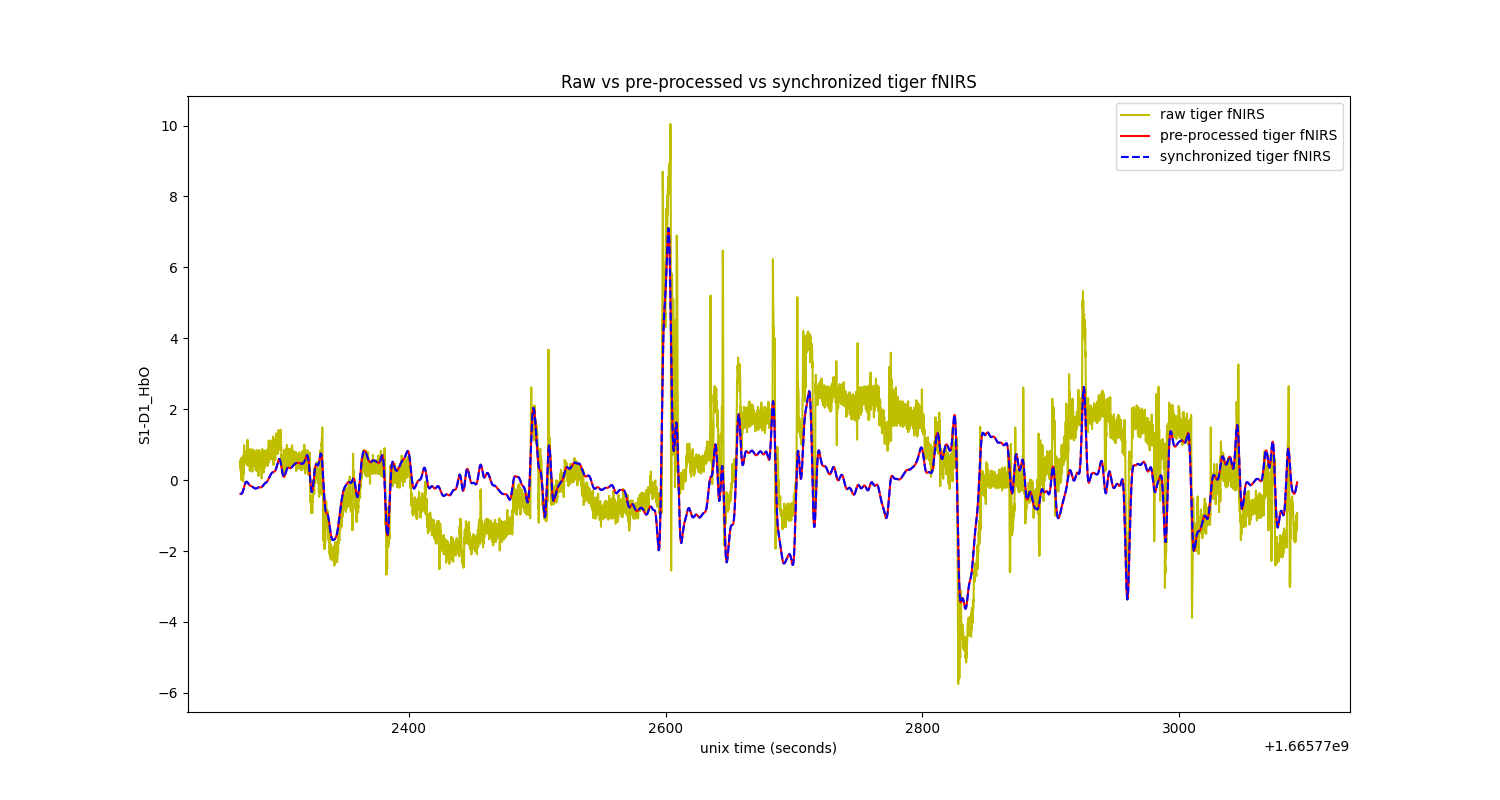
\includegraphics[width=\textwidth]{images/fnirs_filtered}
  \caption{823-second sequence of the fNIRS signals procured from a participant utilizing the Tiger computer, specifically from channel S1-D1\_HbO. Three types of signals are presented: the raw fNIRS signal, the pre-processed signal, and the synchronized signal. The raw signal serves as the baseline, directly acquired from the recording. The pre-processed signal is the result of linear interpolation and bandpass filtering (using a 4th order Butterworth method with a low cutoff bandwidth of 0.01 Hz and a high cutoff bandwidth of 0.2 Hz) of the raw signal, effectively mitigating noise and artifacts. Lastly, the synchronized signal is derived from the pre-processed signal through resampling, ensuring that all data are aligned in time.
}
  \label{fig:fnirs_filtered}
\end{figure}

\begin{figure}[h]
  \centering
  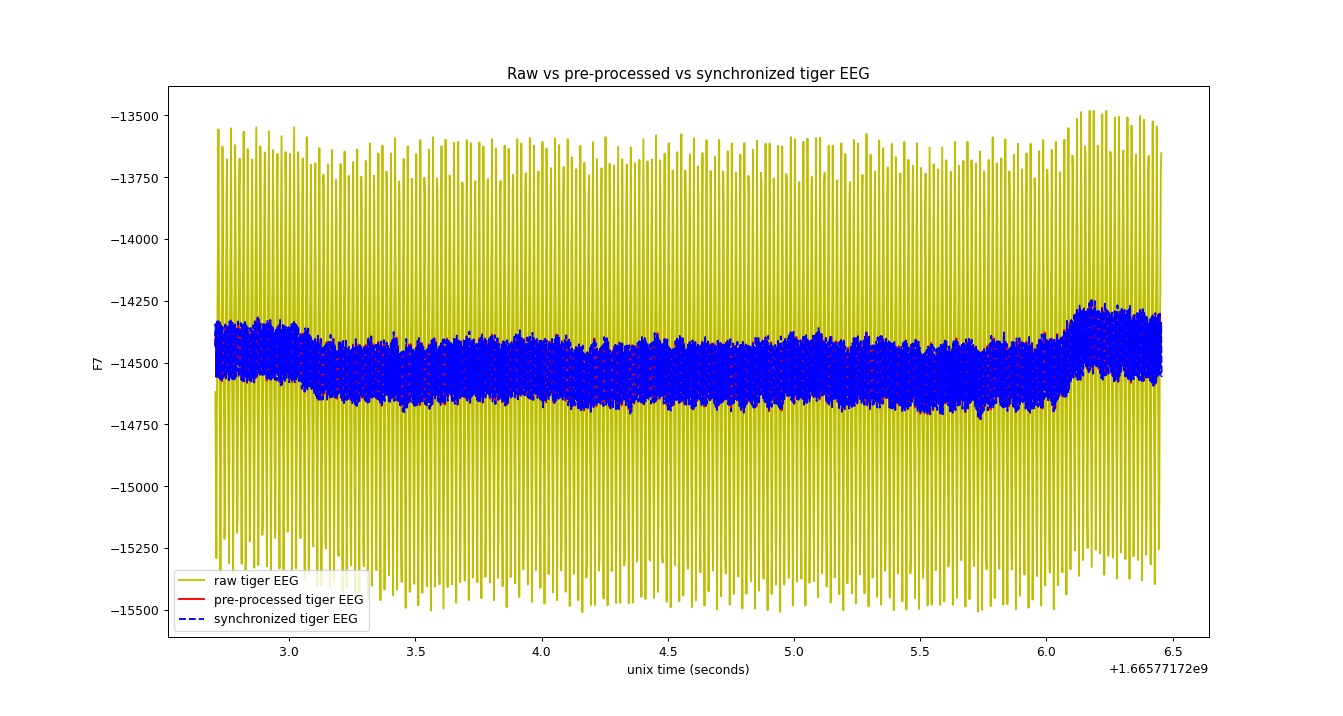
\includegraphics[width=\textwidth]{images/eeg_filtered}
  \caption{3.75-second sequence of the EEG signals gathered from a participant working with the Tiger computer, specifically from channel F7. Three types of signals are presented: the raw EEG signal, the pre-processed signal, and the synchronized signal. The raw signal acts as the baseline, derived directly from the initial recording. The pre-processed signal is derived from the raw signal through linear interpolation and notch filtering (configured at a frequency of 60 Hz, a transition bandwidth of 9 Hz, and notch widths of 2 Hz), effectively reducing noise and artifacts. The synchronized signal, obtained through resampling of the pre-processed signal, assures consistent timing across the experiment.
}
  \label{fig:eeg_filtered}
\end{figure}

\subsection{Synchronizing Task Data with EEG and fNIRS Resampled Signals}

Understanding the relationship between participants' behaviors, environmental stimuli, and neuroimaging data requires a precise synchronization of task data with the corresponding EEG and fNIRS signals. By aligning these data streams, we can examine the influence of environmental stimuli on the participants' neuroimaging signals, which in turn, impact their behavior and task performance.

The process of integrating EEG and fNIRS signals with task data starts with grouping of signals by the tasks during which they were recorded, followed by the synchronization of the task data to the corresponding EEG and fNIRS signals.

\subsubsection{Grouping EEG and fNIRS Signals by Task}

The preliminary step in our approach to synchronizing EEG and fNIRS signals with the task data involves the grouping of EEG and fNIRS signals by the tasks during which the signals were recorded. The task data can be categorized into two distinct types: status-based and event-based data.

\paragraph{Status-based task data} This type of task data represent the current state of the task, such as task score. For each task, the grouping process of these data begins by including the EEG and fNIRS signal recorded immediately before the task initiation and immediately following task completion. This ensures no data is overlooked at the boundaries of the task. Subsequently, all EEG and fNIRS signals recorded between these two points are included, forming a complete set of signals associated with the task.

\paragraph{Event-based task data} This type of task data, on the other hand, correspond to specific events that occur during the task, such as affective task arousal or the submission of a valence score. For each task, we determine the EEG and fNIRS entry associated with the first event and the last event. These signal entries, as well as all entries recorded between these points, are included into the data set related to the task. For the accurate synchronization of event-based data, we ensure that no two or more events are allocated to the same EEG and fNIRS entry, and no event is omitted from the final synchronized data set.

\subsubsection{Synchronizing Task Data with EEG and fNIRS Signals}

Having grouped the EEG and fNIRS signals according to task type, we then proceed to synchronize these signal entries with their respective task data.

\paragraph{Status-based task data} The synchronization is accomplished by assigning the status data recorded closest in time to each EEG and fNIRS signal entry. This method ensures that each EEG and fNIRS entry is paired with the most representative status data.

\paragraph{Event-based task data} We assign each event data to the EEG and fNIRS signal entry recorded at the time closest to the occurrence of the event. Those EEG and fNIRS signal entries without a corresponding event data are left unassigned, signifying that no specific event occurred during these recordings.
